\documentclass{article}
\usepackage[utf8]{inputenc}
\usepackage[margin=1in]{geometry}
\usepackage[titletoc,title]{appendix}
\usepackage{amsmath,amsfonts,amssymb,mathtools}
\usepackage{graphicx,float}
\usepackage[ruled,vlined]{algorithm2e}
\usepackage{algorithmic}
\usepackage{minted}
\usemintedstyle{borland}
\usepackage{biblatex}
\usepackage{subcaption}
\usepackage[table,xcdraw]{xcolor}
\usepackage{verbatim}
\usepackage{multirow}
\usepackage{bm}
\usepackage{listings}
\usepackage{hyperref}
\usepackage{listings}
\usepackage{color} %red, green, blue, yellow, cyan, magenta, black, white
\definecolor{mygreen}{RGB}{28,172,0} % color values Red, Green, Blue
\definecolor{mylilas}{RGB}{170,55,241}
\usepackage{hyperref}
\usepackage{siunitx}
\usepackage{fancyvrb}
\usepackage{tcolorbox}
\newcommand{\Ds}{\mathcal{D}_s}
\newcommand{\Df}{\mathcal{D}_f}
% redefine \VerbatimInput
\RecustomVerbatimCommand{\VerbatimInput}{VerbatimInput}%
{fontsize=\footnotesize,
 %
 frame=lines,  % top and bottom rule only
 framesep=2em, % separation between frame and text
 % rulecolor=\color{Gray},
 %
 % label=\fbox{\color{Black}data.txt},
 labelposition=topline,
 %
 commandchars=\|\(\), % escape character and argument delimiters for
                      % commands within the verbatim
 commentchar=*        % comment character
}
\hypersetup{
    colorlinks=true,
    linkcolor=blue,
    filecolor=magenta,      
    urlcolor=cyan,
}

\usepackage{xcolor}
\definecolor{codegreen}{rgb}{0,0.6,0}
\definecolor{codegray}{rgb}{0.5,0.5,0.5}
\definecolor{codepurple}{rgb}{0.58,0,0.82}
\definecolor{backcolour}{rgb}{0.95,0.95,0.92}

\lstdefinestyle{mystyle}{
    backgroundcolor=\color{backcolour},   
    commentstyle=\color{codegreen},
    keywordstyle=\color{magenta},
    numberstyle=\tiny\color{codegray},
    stringstyle=\color{codepurple},
    basicstyle=\ttfamily\footnotesize,
    breakatwhitespace=false,         
    breaklines=true,                 
    captionpos=b,                    
    keepspaces=true,                 
    numbers=left,                    
    numbersep=5pt,                  
    showspaces=false,                
    showstringspaces=false,
    showtabs=false,                  
    tabsize=2
}


\usepackage{xcolor}

% Define a warm background color (light beige/cream)
% \definecolor{bg}{RGB}{255, 250, 240} % FloralWhite, warm and easy on the eyes
\definecolor{bg}{RGB}{127,127,214} % FloralWhite, warm and easy on the eyes
\colorlet{bg}{bg!15!white} % 15% original color, 85% white
\setminted{
    fontsize=\normalsize,
    linenos,
    breaklines,
    % frame=single,
    framesep=2mm,
    baselinestretch=1.1,
    bgcolor=bg
}


\lstset{style=mystyle}

\addbibresource{references.bib}

% define commands for equation
\def\eq{Eqn.~}
\def\eqs{Eqns.~}
% define commands for figure
\def\fig{Fig.~}
\def\figs{Figs.~}
\def\drm{{\textrm{d}}}
\def\br{{\bf r}}
\def\ppd#1#2{\frac{\partial #1}{\partial #2}}
\def\bn{{\bf n}}
\def\bb{{\bf b}}
\def\ft#1{{\hat {#1}}}
\def\comp#1{\tilde{#1}}
\def\ppdtwo#1#2{\frac{\partial^2 #1}{\partial {#2}^2}}
\def\ppdij#1#2#3{\frac{\partial^2 #1}{\partial #2}{\partial #3}}
\def\dx{\delta x}
\def\dy{\delta y}
\def\dz{\delta z}
\def\al{\alpha}
\def\bi{\mathbf{i}}
\def\bj{\mathbf{j}}
\def\bk{\mathbf{k}}
\def\dd{\delta_d}

\newcommand{\tb}[1]{\textcolor{blue}{#1}}
\newcommand{\tr}[1]{\textcolor{red}{#1}}

\title{Performance Optimization and Profiling of MLPCpp in SU2 \\ GSoC 2025 Final Report}
\author{Divyaprakash}
%\date{}

\begin{document}

\maketitle


\section{Introduction}
\label{sec:intro}

SU2~\cite{economon2016su2} is an open-source suite for computational fluid dynamics (CFD) widely used in both research and 
industrial design. Within SU2, the \texttt{MLPCpp} module provides a compact C++ library for enabling 
multilayer perceptron (MLP) inference as part of solver workflows. This capability supports a range of 
data-driven tasks, including surrogate modeling of fluid properties and inverse regression problems.

The original implementation of \texttt{MLPCpp} contained some performance 
bottlenecks and limitations in usability for advanced data-driven workflows. As part of this Google Summer of Code (GSoC) project, a series of profiling, optimization, and refactoring efforts were undertaken to improve runtime efficiency 
and extend the functionality of the library. Key directions included the introduction of more efficient data 
structures, the refactoring of computational kernels for improved memory locality and numerical precision, 
and enhancements to variable mapping mechanisms to support more complex workflows. 

Profiling was initially conducted with \texttt{gprof}, followed by more detailed analysis with 
\texttt{valgrind} and \texttt{kcachegrind}, and later \texttt{Tracy}, to identify hotspots in the neural 
network inference pipeline. Guided by these insights, multiple optimizations were implemented, ranging 
from memory layout improvements in the weight matrices to function-level optimizations using fused 
multiply-add instructions. In addition, a low-overhead profiling capability was integrated into the SU2 
build system along with documentation to enable future contributors to easily instrument and profile 
the code. 

% \section{Performance Improvement}

\section{Code Profiling and Identifying Bottlenecks}
\label{sec:profile}
Code profiling was initially carried out using the \texttt{gprof} profiler 
that is included with the \texttt{SU2} installation, in order to identify 
the functions contributing most to the overall runtime. However, to obtain 
a clearer picture of the child processes and to determine which operations 
were consuming time within those functions, \texttt{valgrind} and 
\texttt{kcachegrind} were subsequently employed. The latter provided 
an interactive visualization of the profiling data, including call graphs 
and annotated source code views, as shown in Figure~\ref{fig:callgraph}. 
A detailed description of this process was also documented in a 
blog post.\footnote{\url{https://dpcfd.com/posts/2025/06/gsoc-week-2/}}

\begin{figure}[htbp]
    \centering
    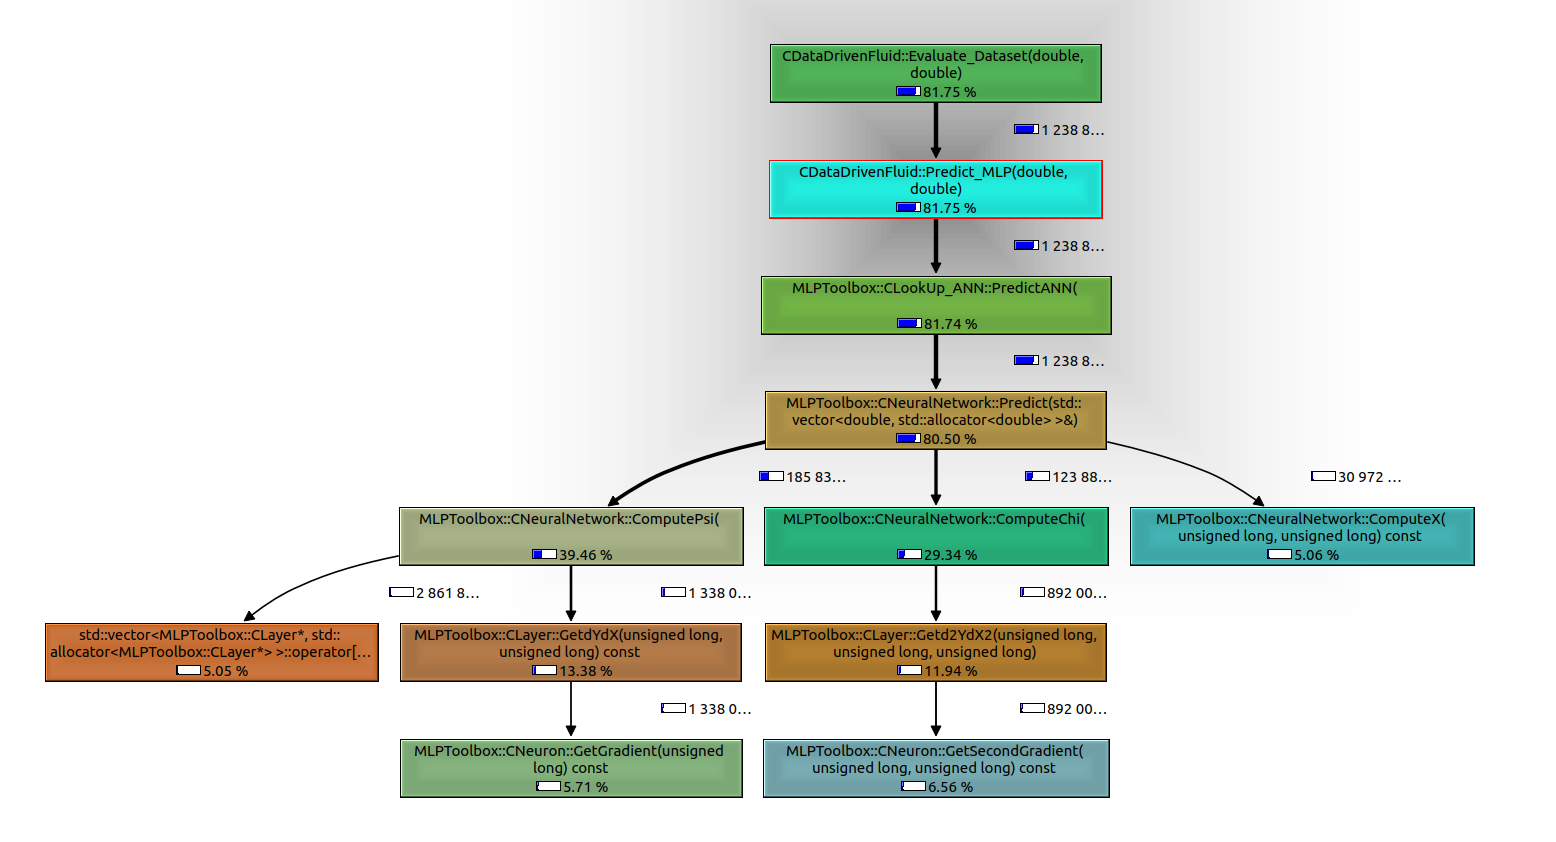
\includegraphics[width=0.8\textwidth]{call_graph.png}
    \caption{Call graph generated using \texttt{valgrind} and \texttt{kcachegrind}. 
    The functions \texttt{ComputePsi}, \texttt{ComputeChi}, and \texttt{ComputeX} 
    were identified as major contributors to the runtime.}
    \label{fig:callgraph}
\end{figure}

From the profiling results, it was observed that the function 
\texttt{Predict} itself did not consume a significant amount of self time. 
Instead, the majority of the runtime was spent in the functions 
\texttt{ComputePsi}, \texttt{ComputeChi}, and \texttt{ComputeX}. 
These functions were therefore identified as the main targets for optimization.

\subsection{Suggested Improvements}

The performance analysis indicated that the loop within 
\texttt{ComputeX} could be made more efficient. A representative code snippet 
is shown below:

\begin{minted}[fontsize=\small, linenos]{cpp}
mlpdouble ComputeX(std::size_t iLayer, std::size_t iNeuron) const {
  mlpdouble x;
  x = total_layers[iLayer]->GetBias(iNeuron);
  std::size_t nNeurons_previous = total_layers[iLayer - 1]->GetNNeurons();
  for (std::size_t jNeuron = 0; jNeuron < nNeurons_previous; jNeuron++) {
    x += weights_mat[iLayer - 1][iNeuron][jNeuron] *
         total_layers[iLayer - 1]->GetOutput(jNeuron);
  }
  return x;
}
\end{minted}

The nested access pattern, arising from the use of a \emph{vector of vectors of vectors}, was found to result in fragmented memory allocation:
\begin{minted}{cpp}
std::vector<std::vector<std::vector<mlpdouble>>> weights_mat;
\end{minted}
To improve performance, this structure was modified, with the changes and their effects described in the following sections.

\subsection{Advanced Profiling with Tracy}

In addition to \texttt{valgrind}, another profiling option was later 
explored, namely \texttt{Tracy}, which offers very low overhead and provides 
fine-grained insights into performance. This profiler was integrated with the 
\texttt{meson} build system of \texttt{SU2}, and changes were made to the 
\texttt{SU2} codebase to facilitate easy instrumentation. Both the integration 
and the accompanying documentation were contributed as two separate Pull Requests 
as part of this GSoC project.\footnote{\url{https://github.com/su2code/SU2/pull/2536}}%
\footnote{\url{https://github.com/su2code/su2code.github.io/pull/180}}

\section{Optimizing Weights Matrix Storage}
\label{sec:weights}
From the above discussions, it has been well established that one way to optimize the code is by improving how the weight matrices are stored. Currently, they are implemented as 3D nested vectors. To enhance performance, we consider two alternative approaches: replacing the 3D nested vectors with raw 3D pointers, or using flattened vectors. The implementation and results of both approaches are presented in the following subsections. Before that, however, we first review the current implementation of the weight matrix.

\subsection{Weights Matrix}
Before modifying the implementation of the weights matrix, it is important to understand the existing design. Neural networks stored in \texttt{.mlp} files follow the TensorFlow convention, where weights are arranged as \emph{source $\times$ destination}. In contrast, traditional mathematical notation typically uses the \emph{destination $\times$ source} order. This difference is illustrated in Figure~\ref{fig:wmat}.

The \texttt{MLPCpp} code addresses this discrepancy in a clean manner:  
\begin{enumerate}
    \item \texttt{CReadNeuralNetwork::weights\_mat} serves as a temporary container inside the reader class. It parses the \texttt{.mlp} file and stores the weights exactly as they appear.
    \item \texttt{CNeuralNetwork::weights\_mat} belongs to the functional network class. Here, the matrix is transposed to match the conventional layout and is used in the \texttt{Predict} method for evaluation.
\end{enumerate}

The key reason for this layout is computational efficiency. CPUs favor memory locality: they are significantly faster when reading data stored contiguously. Consider the dot product inside the \texttt{ComputeX} function:

\begin{minted}{cpp}
// Core computation of the network
for (std::size_t jNeuron = 0; jNeuron < nNeurons_previous; jNeuron++) {
    x += weights_mat[iLayer - 1][iNeuron][jNeuron] *
         total_layers[iLayer - 1]->GetOutput(jNeuron);
}
\end{minted}

Here, the input for a destination neuron (\texttt{iNeuron}) is computed by iterating through all source neurons (\texttt{jNeuron}). With the current \texttt{[layer][destination][source]} storage, all weights for a given destination neuron are contiguous in memory. During iteration, the CPU accesses them sequentially. 

From the above discussions, it is concluded that any modification to the weight matrix storage for performance benefits must be applied to \texttt{CNeuralNetwork::weights\_mat}.

\begin{figure}[ht]
\begin{subfigure}{.5\textwidth}
  \centering
  % include first image
  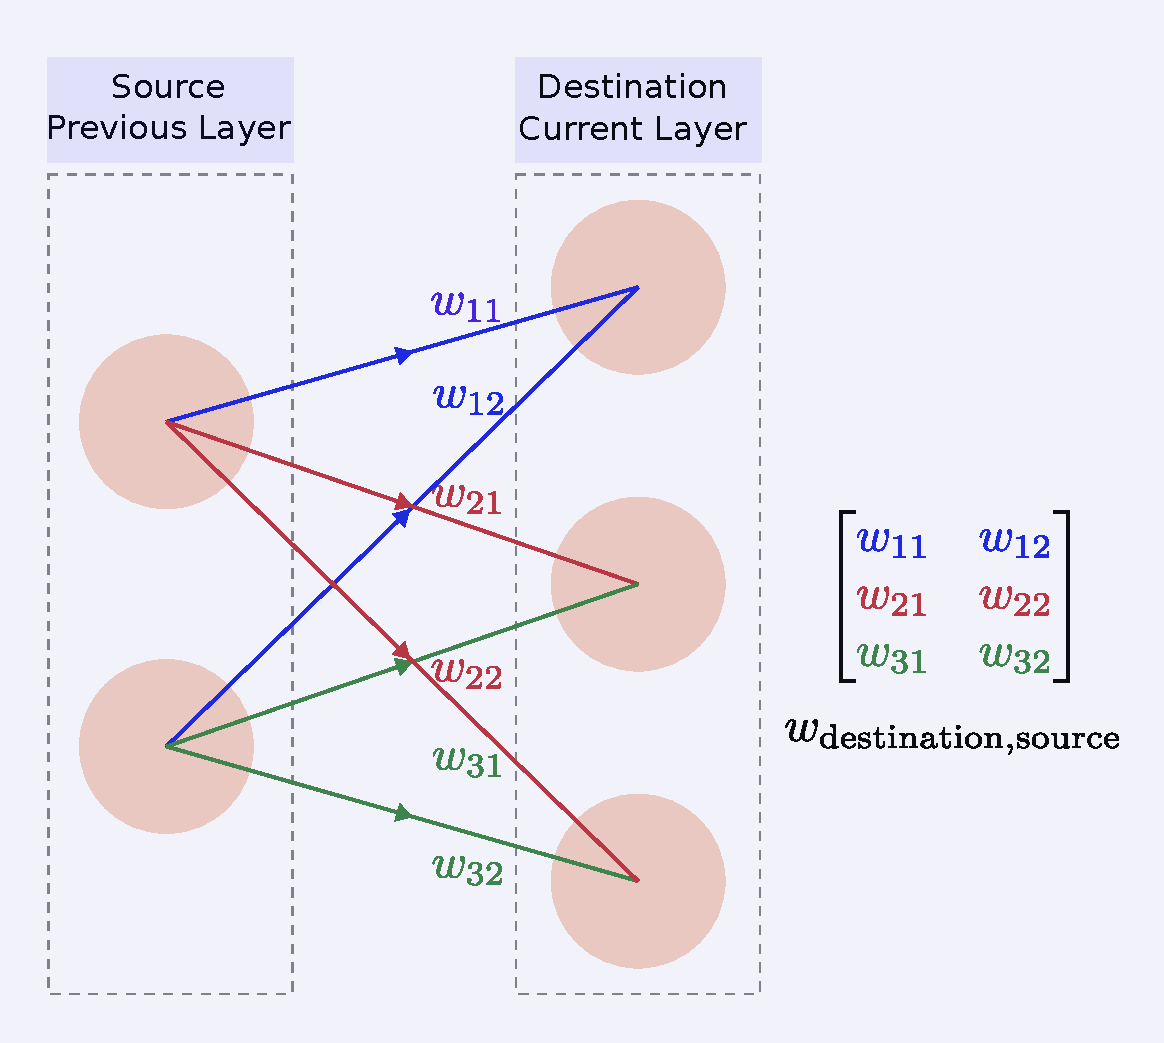
\includegraphics[width=.9\linewidth]{nn_keras.pdf}  
  \caption{Conventional}
  \label{fig:conv}
\end{subfigure}
\begin{subfigure}{.5\textwidth}
  \centering
  % include second image
  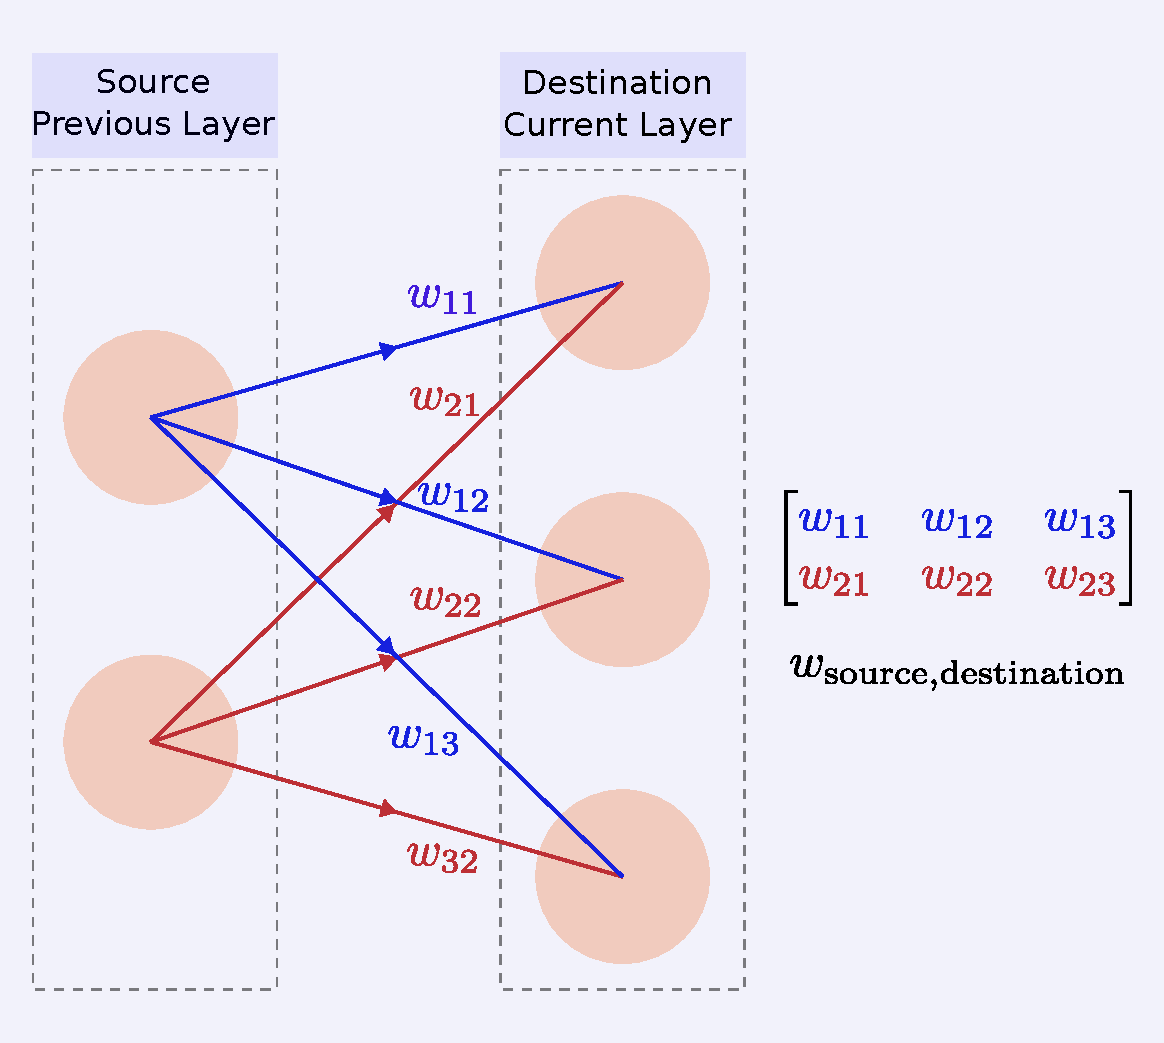
\includegraphics[width=.9\linewidth]{nn.pdf}  
  \caption{Tensorflow}
  \label{fig:tf}
\end{subfigure}
\caption{Comparison of weight matrix arrangements in neural networks: conventional mathematical notation (a) versus TensorFlow implementation (b). The diagrams show connections between a 2-neuron source layer and a 3-neuron destination layer, with corresponding weight matrix dimensions and indexing conventions.}
\label{fig:wmat}
\end{figure}

\subsection{3D Pointer}
\label{subsec:3D}
The neural network implementation previously employed a three-dimensional vector to represent the weight matrix.
\[
\texttt{std::vector<std::vector<std::vector<mlpdouble>>> weights\_mat}
\]
While convenient, this approach introduced additional overhead and less predictable memory access patterns. To optimize performance and provide finer control over memory allocation, the structure has been refactored to use a triple pointer, declared as
\[
\texttt{mlpdouble*** weights\_mat}
\]

\subsubsection{Implementation}
The refactored design maintains the logical indexing scheme 
\[
\texttt{weights\_mat[layer][destination][source]}
\]
while eliminating the overhead of nested \texttt{std::vector} containers. Allocation proceeds hierarchically:
\begin{enumerate}
  \item An array of pointers for each layer.
  \item For each layer, an array of neuron pointers.
  \item For each neuron, an array of incoming weights.
\end{enumerate}
It is implemented as follows in the \texttt{SizeWeights()} Function.
\begin{minted}{cpp}
    weights_mat = new mlpdouble**[n_hidden_layers + 1];
    weights_mat[0] = new mlpdouble*[hiddenLayers[0]->GetNNeurons()];
    for (auto iNeuron = 0u; iNeuron < hiddenLayers[0]->GetNNeurons(); iNeuron++)
      weights_mat[0][iNeuron] = new mlpdouble[inputLayer->GetNNeurons()];

    for (auto iLayer = 1u; iLayer < n_hidden_layers; iLayer++) {
      weights_mat[iLayer] = new mlpdouble*[hiddenLayers[iLayer]->GetNNeurons()];
      for (auto iNeuron = 0u; iNeuron < hiddenLayers[iLayer]->GetNNeurons();
           iNeuron++) {
        weights_mat[iLayer][iNeuron] = new mlpdouble[hiddenLayers[iLayer - 1]->GetNNeurons()];
      }
    }
    weights_mat[n_hidden_layers] = new mlpdouble*[outputLayer->GetNNeurons()];
    for (auto iNeuron = 0u; iNeuron < outputLayer->GetNNeurons(); iNeuron++) {
      weights_mat[n_hidden_layers][iNeuron] = new mlpdouble[hiddenLayers[n_hidden_layers - 1]->GetNNeurons()];
    }

    ANN_outputs = new mlpdouble[outputLayer->GetNNeurons()];
\end{minted}

% \subsection{Memory Management}
Because allocation is manual, explicit deallocation must follow the inverse order:
\begin{enumerate}
  \item Deallocate each neuron's incoming weights.
  \item Deallocate each layer's array of neuron pointers.
  \item Finally, deallocate the outer layer array.
\end{enumerate}
This approach ensures memory safety and prevents leaks. The updated destructor is given below:

\begin{minted}{cpp}
~CNeuralNetwork() {
    delete[] ANN_outputs;
   
    if (weights_mat != nullptr) {
        // Clean up first layer (input to first hidden)
        if (n_hidden_layers > 0) {
            for (auto iNeuron = 0u; iNeuron < hiddenLayers[0]->GetNNeurons(); iNeuron++) {
                delete[] weights_mat[0][iNeuron];
            }
            delete[] weights_mat[0];
        }
       
        // Clean up hidden layers
        for (auto iLayer = 1u; iLayer < n_hidden_layers; iLayer++) {
            for (auto iNeuron = 0u; iNeuron < hiddenLayers[iLayer]->GetNNeurons(); iNeuron++) {
                delete[] weights_mat[iLayer][iNeuron];
            }
            delete[] weights_mat[iLayer];
        }
       
        // Clean up last layer (last hidden to output)
        if (outputLayer != nullptr) {
            for (auto iNeuron = 0u; iNeuron < outputLayer->GetNNeurons(); iNeuron++) {
                delete[] weights_mat[n_hidden_layers][iNeuron];
            }
            delete[] weights_mat[n_hidden_layers];
        }
       
        delete[] weights_mat;
    }
   
    delete inputLayer;
    delete outputLayer;
    for (std::size_t i = 1; i < total_layers.size() - 1; i++) {
        delete total_layers[i];
    }
};
\end{minted}

The conversion from \texttt{std::vector} to a triple-pointer preserves the computational logic while improving control over allocation. Public interfaces remain unchanged, so expressions such as \texttt{weights\_mat[i][j][k]} continue to function as before. The main trade-off is between safety and performance: the vector-based implementation offered automatic memory management and bounds checking, whereas the pointer-based design requires careful allocation and deallocation. However, it may provide performance benefits due to reduced overhead and improved cache locality.
\\
\\
\noindent\textbf{Implementation Note:} The complete source code for this refactoring approach is available in the \texttt{$\text{gsoc\_dp}$} branch of the project repository\footnote{\url{https://github.com/divyaprakash-iitd/MLPCpp/tree/gsoc_dp}}.
\subsection{Flattened Vector}
\label{subsec:flat}
\begin{tcolorbox}[colback=bg,colframe=red!60!black,title=Disclaimer]
Some of the changes described in this section are still under debugging and may not yet work as intended.
\end{tcolorbox}
In this section, an alternative approach is proposed to refactor the core weight storage from a 3D \texttt{std::vector} of vectors to a single, contiguous, flattened 1D \texttt{std::vector} for improved performance. The refactoring is to be performed in three safe, verifiable phases:
\begin{enumerate}
    \item \textbf{Parallel Implementation:} Introduce the new flattened vector and its accessor functions \emph{alongside} the existing implementation.
    \item \textbf{Verification:} Run both the original \texttt{Predict} function and a new \texttt{Predict\_flat} function to check if the new implementation is mathematically identical.
    \item \textbf{Cleanup:} Once verification is successful, the old 3D vector and its associated functions are removed.
\end{enumerate}

\subsubsection{Implementation}
This phase involves adding new code without modifying the existing, validated logic.
\paragraph{Step 1: Modify \texttt{CNeuralNetwork.hpp} - Data Structures \& Accessors:}

New data structures and accessor functions are added to the \texttt{CNeuralNetwork} class. In the \texttt{private} section of the \texttt{CNeuralNetwork} class, new variables are added:

\begin{minted}{cpp}
// Add this block in the private section of CNeuralNetwork
// --- New flattened vector implementation ---
std::vector<mlpdouble> flat_weights;
std::vector<int> layer_sizes;
std::vector<int> layer_offsets;
\end{minted}

New private and public helper functions are added below. These functions utilize the \texttt{inline} keyword to ensure compiler optimization eliminates function call overhead when optimizations are enabled (e.g., with the \texttt{-O2} flag).

\begin{minted}{cpp}
// Add this function to the private section of CNeuralNetwork
/**
 * @brief (NEW) Calculates the 1D index for the flattened weights vector.
 */
inline int get_flat_index(int i_layer, int i_dest_neuron, int i_src_neuron) const {
    return layer_offsets[i_layer] + i_dest_neuron * layer_sizes[i_layer] + i_src_neuron;
}

// Add these functions to the public section of CNeuralNetwork
/**
 * @brief (NEW) Sets a weight value in the flattened vector, handling the index swap.
 */
inline void SetFlatWeight(unsigned long i_layer, unsigned long i_src_neuron, 
                         unsigned long i_dest_neuron, mlpdouble value) {
    int index = get_flat_index(i_layer, i_dest_neuron, i_src_neuron);
    flat_weights[index] = value;
}

/**
 * @brief (NEW) Gets a weight value from the flattened vector using the in-memory layout.
 */
inline mlpdouble GetFlatWeight(int i_layer, int i_dest_neuron, int i_src_neuron) const {
    return flat_weights[get_flat_index(i_layer, i_dest_neuron, i_src_neuron)];
}
\end{minted}

\paragraph{Step 2: Modify \texttt{CNeuralNetwork.hpp} - Sizing the New Structures:}

In the \texttt{SizeWeights()} function, logic is added to calculate the total number of weights and correctly size the new helper vectors and the \texttt{flat\_weights} vector.

\begin{minted}{cpp}
// In CNeuralNetwork.hpp
void SizeWeights() {
    // ... existing code to set up total_layers ...

    // --- START NEW IMPLEMENTATION ---
    layer_sizes.clear();
    for(const auto& layer : total_layers) {
        layer_sizes.push_back(layer->GetNNeurons());
    }

    layer_offsets.clear();
    int total_weights = 0;
    layer_offsets.push_back(total_weights);

    for (size_t i = 0; i < GetNLayers() - 1; ++i) {
        int weights_in_layer = layer_sizes[i+1] * layer_sizes[i];
        total_weights += weights_in_layer;
        layer_offsets.push_back(total_weights);
    }
    flat_weights.resize(total_weights);
    // --- END NEW IMPLEMENTATION ---

    // --- OLD IMPLEMENTATION (unchanged for now) ---
    weights_mat.resize(n_hidden_layers + 1);
    // ... (rest of the old implementation)
}
\end{minted}

\paragraph{Step 3: Modify \texttt{CLookUp\_ANN.hpp} - Populating Both Data Structures:}

This represents the only change needed for the data loading part of the refactoring. In the \texttt{CLookUp\_ANN} class, within the nested loop that sets the weights, a call to the new \texttt{SetFlatWeight} function is added. The \texttt{Reader} object has already parsed the \texttt{.ann} file into its own memory. This loop transfers that data into the \texttt{ANN} object used for computations. A line is simply added to populate the new \texttt{flat\_weights} vector simultaneously with the original \texttt{weights\_mat}.

\begin{minted}{cpp}
// In CLookUp_ANN.hpp, inside the constructor or loading function, around line 108
for (auto i_layer = 0u; i_layer < ANN.GetNWeightLayers(); i_layer++) {
  ANN.SetActivationFunction(i_layer, Reader.GetActivationFunction(i_layer));
  for (auto i_neuron = 0u; i_neuron < ANN.GetNNeurons(i_layer); i_neuron++) {
    for (auto j_neuron = 0u; j_neuron < ANN.GetNNeurons(i_layer + 1); j_neuron++) {
      
      // Original call (unchanged)
      ANN.SetWeight(i_layer, i_neuron, j_neuron,
                    Reader.GetWeight(i_layer, i_neuron, j_neuron));

      // --- ADD THIS LINE ---
      // New call to populate the parallel flat vector structure
      ANN.SetFlatWeight(i_layer, i_neuron, j_neuron,
                        Reader.GetWeight(i_layer, i_neuron, j_neuron));
      // ---------------------
    }
  }
}
\end{minted}

\paragraph{Step 4: Modify \texttt{CNeuralNetwork.hpp} - Create Parallel Compute Functions:}

For every function that uses \texttt{weights\_mat}, a duplicate version with a \texttt{\_flat} suffix is created that uses the new \texttt{GetFlatWeight} accessor.

\begin{minted}{cpp}
// In CNeuralNetwork.hpp, add these new functions.

/**
 * @brief (NEW) Compute neuron activation function input using the flattened weights.
 */
mlpdouble ComputeX_flat(std::size_t iLayer, std::size_t iNeuron) const {
      mlpdouble x = total_layers[iLayer]->GetBias(iNeuron);
      std::size_t nNeurons_previous = total_layers[iLayer - 1]->GetNNeurons();
      for (std::size_t jNeuron = 0; jNeuron < nNeurons_previous; jNeuron++) {
          // Access is [layer][destination][source]
          x += GetFlatWeight(iLayer - 1, iNeuron, jNeuron) *
               total_layers[iLayer - 1]->GetOutput(jNeuron);
      }
      return x;
  }


/**
 * @brief (NEW) Compute Psi for gradients using the flattened weights.
 */
mlpdouble ComputePsi_flat(std::size_t iLayer, std::size_t iNeuron, 
                                std::size_t jInput) const { 
    // Implementation using GetFlatWeight...
}

// ... and so on for ComputeChi, etc. ...
\end{minted}


Once verification with the flattened implementations is successful, the old implementation can be safely removed. After these steps, the project is fully migrated to the new, more efficient flattened weight structure, providing improved memory locality and cache performance for neural network computations.
\\
\\
\noindent\textbf{Implementation Note:} The complete source code for this refactoring approach is available in the \texttt{flatten} branch of the project repository\footnote{\url{https://github.com/divyaprakash-iitd/MLPCpp/tree/flatten}}.

\section{Optimizing Variable Matching}
\label{sec:varmatch}
Efficient mapping of input and output variables is essential for integrating neural networks within \texttt{MLPCpp}. A hash map–based method, along with a cleaner replacement for the \texttt{FindVariableIndices} function, was proposed to improve clarity and maintainability.


\subsection{Hash Maps}
\label{subsec:hash}
The changes were made to the \texttt{FindVariableIndices} function. This function is responsible for mapping variable names to their corresponding indices within the Artificial Neural Network (ANN).

The original implementation used a nested loop structure to find matching variable names. The outer loop iterated through the variables of the ANN, and the inner loop iterated through the list of variable names to be found. This approach has a time complexity of $O(N \times M)$, where N is the number of variables in the ANN and M is the number of variables to be mapped. For large models, this can lead to significant performance bottlenecks.

\subsubsection{Implementation}
The new implementation in \texttt{CLookUp\_ANN.hpp} replaces the nested loops with a more efficient approach utilizing a \texttt{std::unordered\_map} (hash map). The steps are as follows:

\begin{enumerate}
    \item A hash map is created, mapping each variable name to its index in the input list.
    \item The code then iterates a single time through the ANN\'s variables.
    \item For each ANN variable, it performs a quick lookup in the hash map to see if there is a match.
\end{enumerate}

This change reduces the time complexity to $O(N+M)$, which is a substantial improvement over the previous $O(N \times M)$.

\begin{minted}{cpp}
  std::vector<std::pair<size_t, size_t>> FindVariableIndices(
    std::size_t i_ANN,
    std::vector<std::string> variable_names,
    bool input) const {
    std::vector<std::pair<size_t, size_t>> variable_indices;
    auto nVar = input ? NeuralNetworks[i_ANN].GetnInputs()
                      : NeuralNetworks[i_ANN].GetnOutputs();

    // Create a hash map from variable names to their indices
    std::unordered_map<std::string, size_t> name_to_index;
    for (size_t jVar = 0; jVar < variable_names.size(); ++jVar) {
        name_to_index[variable_names[jVar]] = jVar;
    }

    // Iterate over neural network variables
    for (size_t iVar = 0; iVar < nVar; ++iVar) {
        std::string ANN_varname = input ? NeuralNetworks[i_ANN].GetInputName(iVar)
                                       : NeuralNetworks[i_ANN].GetOutputName(iVar);
        // Look up the variable name in the hash map
        auto it = name_to_index.find(ANN_varname);
        if (it != name_to_index.end()) {
            variable_indices.push_back(std::make_pair(it->second, iVar));
        }
    }

    return variable_indices;
}
\end{minted}

The new implementation offers several advantages:
\begin{itemize}
    \item \textbf{Improved Performance:} The use of a hash map for lookups is significantly faster than the nested loop approach, especially as the number of variables increases.
    \item \textbf{Enhanced Readability:} The new code is more organized and easier to understand. The logic is more straightforward, which improves maintainability.
    \item \textbf{Better Scalability:} The improved performance ensures that the code will scale more effectively as the complexity of the neural network models grows.
\end{itemize}
\noindent\textbf{Implementation Note:} The complete source code for this refactoring approach is available in the \texttt{$\text{gsoc\_dp}$} branch of the project repository\footnote{\url{https://github.com/divyaprakash-iitd/MLPCpp/tree/gsoc_dp}}.

\subsection{Replacing \texttt{FindVariableIndices} Function}
\label{subsec:varmap2}
\begin{tcolorbox}[colback=bg,colframe=red!60!black,title=Disclaimer]
Some of the changes described in this section are still under debugging and may not yet work as intended.
\end{tcolorbox}
In this section, an alternative approach is proposed for refactoring of the variable matching logic within the \texttt{CLookUp\_ANN} and \texttt{CNeuralNetwork} classes. The goal is to improve \textbf{efficiency, readability, and maintainability}. The key change is to replace the current \texttt{FindVariableIndices} function with a more powerful and efficient method, \texttt{GetVariableMapping}, inside the \texttt{CNeuralNetwork} class. This new method performs the complete variable matching and index retrieval in a single operation, eliminating redundant work and clarifying the code's intent.

The original implementation in \texttt{CLookUp\_ANN::PairVariableswithMLPs} relied on calling \texttt{FindVariableIndices} twice (once for inputs, once for outputs) for every neural network in the collection.

\begin{minted}{cpp}
// Original logic
std::vector<std::pair<size_t, size_t>> Input_Indices =
    FindVariableIndices(iMLP, inputVariables, true);
isInput = Input_Indices.size() > 0;

if (isInput) {
  std::vector<std::pair<size_t, size_t>> Output_Indices =
      FindVariableIndices(iMLP, outputVariables, false);
  isOutput = Output_Indices.size() > 0;

  if (isOutput) {
    // ... update map
  }
}
\end{minted}

This approach has two main drawbacks:
\begin{enumerate}
    \item \textbf{Inefficiency:} It involves multiple loops and lookups for a single network check.
    \item \textbf{Separation of Concerns:} The logic for how a \texttt{CNeuralNetwork} matches against a set of variables was located in the \texttt{CLookUp\_ANN} class, not within the \texttt{CNeuralNetwork} class itself.
\end{enumerate}

While \texttt{operator==} was suggested, it is not ideal because it's expected to return a simple \texttt{bool}, whereas this operation requires the resulting index maps. A boolean check would still require a second operation to retrieve the indices, leading to redundant computation.

\subsubsection{Implementation}

The proposed solution centralizes the matching logic into a single, efficient method within the \texttt{CNeuralNetwork} class.

\paragraph{Step 1: Introduce \texttt{MatchResult} Struct and \texttt{GetVariableMapping} Method}

A new struct, \texttt{MatchResult}, is defined to hold the complete result of a matching operation. A new public method, \texttt{GetVariableMapping}, is added to \texttt{CNeuralNetwork}.

\begin{minted}{cpp}
// CNeuralNetwork.hpp
// Add this struct definition before the CNeuralNetwork class
struct MatchResult {
    bool is_match = false;
    std::vector<std::pair<size_t, size_t>> input_indices;
    std::vector<std::pair<size_t, size_t>> output_indices;
};

// Add this public method to the CNeuralNetwork class
public:
  MatchResult GetVariableMapping(
      const std::vector<std::string>& lookup_inputs,
      const std::vector<std::string>& lookup_outputs
  ) const;
\end{minted}

This method efficiently checks for matches and returns the \texttt{MatchResult} struct containing a boolean flag and the corresponding index vectors, all in one pass. The matching logic used if given below. 
\begin{itemize}
    \item \textbf{Inputs:} All of the network's defined inputs must be present in the \texttt{lookup\_inputs}.
    \item \textbf{Outputs:} At least one of the network's defined outputs must be present in the \texttt{lookup\_outputs}.
\end{itemize}

\paragraph{Step 2: Simplify \texttt{PairVariableswithMLPs} and Remove \texttt{FindVariableIndices}}

The \texttt{PairVariableswithMLPs} function in \texttt{CLookUp\_ANN.hpp} is refactored to use the new method, making it significantly cleaner and more expressive. The \texttt{FindVariableIndices} function is no longer needed and should be deleted.

\begin{minted}{cpp}
// CLookUp_ANN.hpp
// Replace the old PairVariableswithMLPs function with this:
void PairVariableswithMLPs(MLPToolbox::CIOMap &ioMap) {
    auto inputVariables = ioMap.GetInputVars();
    auto outputVariables = ioMap.GetOutputVars();

    for (size_t iMLP = 0; iMLP < NeuralNetworks.size(); iMLP++) {
      // Single, efficient call to the new method
      auto mapping_result =
          NeuralNetworks[iMLP].GetVariableMapping(inputVariables, outputVariables);

      if (mapping_result.is_match) {
        // Update the map directly with the results
        ioMap.PushMLPIndex(iMLP);
        ioMap.PushInputIndices(mapping_result.input_indices);
        ioMap.PushOutputIndices(mapping_result.output_indices);
      }
    }

    CheckUseOfInputs(ioMap);
    CheckUseOfOutputs(ioMap);
}

// The FindVariableIndices function should be deleted from this file.
\end{minted}

Implementing these changes is expected to yield the following advantages:
\begin{itemize}
    \item \textbf{Efficiency:} Eliminates redundant loops and string comparisons by performing the variable check and index retrieval in a single, optimized operation.
    \item \textbf{Readability:} The code in \texttt{PairVariableswithMLPs} now clearly expresses its intent: get the variable mapping from the network and use it if there is a match.
    \item \textbf{Encapsulation:} The logic for how a neural network matches variables is now correctly placed within the \texttt{CNeuralNetwork} class, improving code organization and maintainability.
\end{itemize}

\noindent\textbf{Implementation Note:} The complete source code for this refactoring approach is available in the \texttt{revarmap} branch of the project repository\footnote{\url{https://github.com/divyaprakash-iitd/MLPCpp/tree/revarmap}}.

\section{Neural Network Function Optimization}
\label{sec:nnfunc}
Several critical computational functions in the neural network implementation were optimized to improve both performance and numerical precision. The optimizations focused on reducing redundant array access operations and leveraging fused multiply-add (FMA) instructions for better floating-point accuracy.

\subsection{Implementation}
The key optimization strategies used are listed below.
\begin{enumerate}
  \item \textbf{Pre-extraction of frequently accessed data}: Weight vectors and neuron counts are cached before loops to minimize repeated pointer dereferencing.
  \item \textbf{FMA instruction usage}: Replaced separate multiplication and addition operations with \texttt{std::fma()} for improved numerical precision and potential performance gains.
  \item \textbf{Consistent variable naming}: Standardized loop indices to improve code readability and maintainability.
\end{enumerate}

Using the above strategies, the following compute functions were optimized. 

\paragraph{ComputeX Function:}
The \texttt{ComputeX} function computes the weighted sum input to a neuron's activation function:

\begin{minted}[fontsize=\small,breaklines]{cpp}
mlpdouble ComputeX(std::size_t iLayer, std::size_t iNeuron) const noexcept {
  const auto& w = weights_mat[iLayer - 1][iNeuron];
  const auto  n = total_layers[iLayer - 1]->GetNNeurons();

  mlpdouble x = total_layers[iLayer]->GetBias(iNeuron); // start from bias
  for (std::size_t j = 0; j < n; ++j) {
    // If GetOutput(j) is cheap (non-virtual, inlined), this is fine.
    x = std::fma(w[j], total_layers[iLayer - 1]->GetOutput(j), x);
  }
  return x;
}
\end{minted}

\paragraph{ComputePsi Function:}
The \texttt{ComputePsi} function computes the weighted sum of output derivatives from the previous layer:

\begin{minted}[fontsize=\small,breaklines]{cpp}
mlpdouble ComputePsi(std::size_t iLayer, std::size_t iNeuron,
                     std::size_t jInput) const
{
    const auto* prev = total_layers[iLayer - 1];                // cache pointer
    const std::size_t n = prev->GetNNeurons();                  // cache bound
    const auto& wrow = weights_mat[iLayer - 1][iNeuron];        // one row of weights

    mlpdouble psi = 0;
    for (std::size_t j = 0; j < n; ++j) {
        psi = std::fma(wrow[j], prev->GetdYdX(j, jInput), psi);
    }
    return psi;
}
\end{minted}

\paragraph{ComputeChi Function:}
The \texttt{ComputeChi} function computes the weighted sum of second-order derivatives from the previous layer:

\begin{minted}[fontsize=\small,breaklines]{cpp}
mlpdouble ComputeChi(std::size_t iLayer, std::size_t iNeuron,
                     std::size_t jInput, std::size_t kInput) const {
  mlpdouble chi = 0;
  for (std::size_t jNeuron = 0;
       jNeuron < total_layers[iLayer - 1]->GetNNeurons();
       ++jNeuron) {
    chi = std::fma(
        weights_mat[iLayer - 1][iNeuron][jNeuron],
        total_layers[iLayer - 1]->Getd2YdX2(jNeuron, jInput, kInput),
        chi);
  }
  return chi;
}
\end{minted}

\paragraph{ComputedOutputdInput Function:}
The \texttt{ComputedOutputdInput} function computes the weighted sum of output derivatives with respect to inputs:

\begin{minted}[fontsize=\small,breaklines]{cpp}
mlpdouble ComputedOutputdInput(std::size_t iLayer, std::size_t iNeuron,
                               std::size_t iInput) const {
  const auto& w = weights_mat[iLayer - 1][iNeuron];
  const auto  n = total_layers[iLayer - 1]->GetNNeurons();
  
  mlpdouble doutput_dinput = 0;
  for (std::size_t j = 0; j < n; ++j) {
    doutput_dinput = std::fma(w[j], total_layers[iLayer - 1]->GetdYdX(j, iInput), doutput_dinput);
  }
  return doutput_dinput;
}
\end{minted}

% \subsection{Discussion}

The use of \texttt{std::fma()} provides improved floating-point precision by performing the multiply-add operation as a single step, reducing intermediate rounding errors that would occur in separate multiplication and addition operations. 

\paragraph{Memory Access Optimization:}
Pre-extracting weight vectors and neuron counts reduces the computational overhead of repeated array indexing and function calls within tight loops, particularly beneficial for networks with large layer sizes.

\paragraph{Cache Efficiency:}
The optimized access patterns improve cache locality by reducing the number of pointer dereferences and enabling more predictable memory access patterns during the forward and backward propagation phases.
\\
\\
\noindent\textbf{Implementation Note:} The complete source code for this refactoring approach is available in the \texttt{$\text{gsoc\_dp}$} branch of the project repository\footnote{\url{https://github.com/divyaprakash-iitd/MLPCpp/tree/gsoc_dp}}.

\section{Results}
\label{sec:results}

The optimizations described in Section~\ref{sec:nnfunc} and 
Subsections~\ref{subsec:3D} and~\ref{subsec:hash} were combined in the code. 
The resulting implementation was submitted as a Pull Request\footnote{\url{https://github.com/EvertBunschoten/MLPCpp/pull/2}} 
to the \texttt{MLPCpp} subproject of \texttt{SU2}. 

To verify the correctness of the implementation, the code was compiled and the 
test case provided in the \texttt{MLPCpp} repository was executed. In this test, 
the derivatives obtained using finite differences were found to agree with those 
calculated analytically by the network, thereby confirming the validity of the implementation.

The prediction times of the original implementation were compared with those of 
the optimized GSoC version over multiple runs. The original implementation was 
observed to have an average runtime of \textbf{251.98~$\pm$~7.16~ms}, whereas the 
optimized version reduced this to \textbf{178.96~$\pm$~4.56~ms}. This corresponds 
to a \textbf{1.41$\times$ speedup}, or equivalently a \textbf{28.9\% reduction in 
execution time}. Figure~X presents the average runtimes with standard deviation 
error bars, which reflect the run-to-run fluctuations in the measurements. It may 
therefore be concluded that the optimized implementation not only achieves faster 
predictions but also exhibits greater consistency across runs.


\begin{figure}[ht]
    \centering
    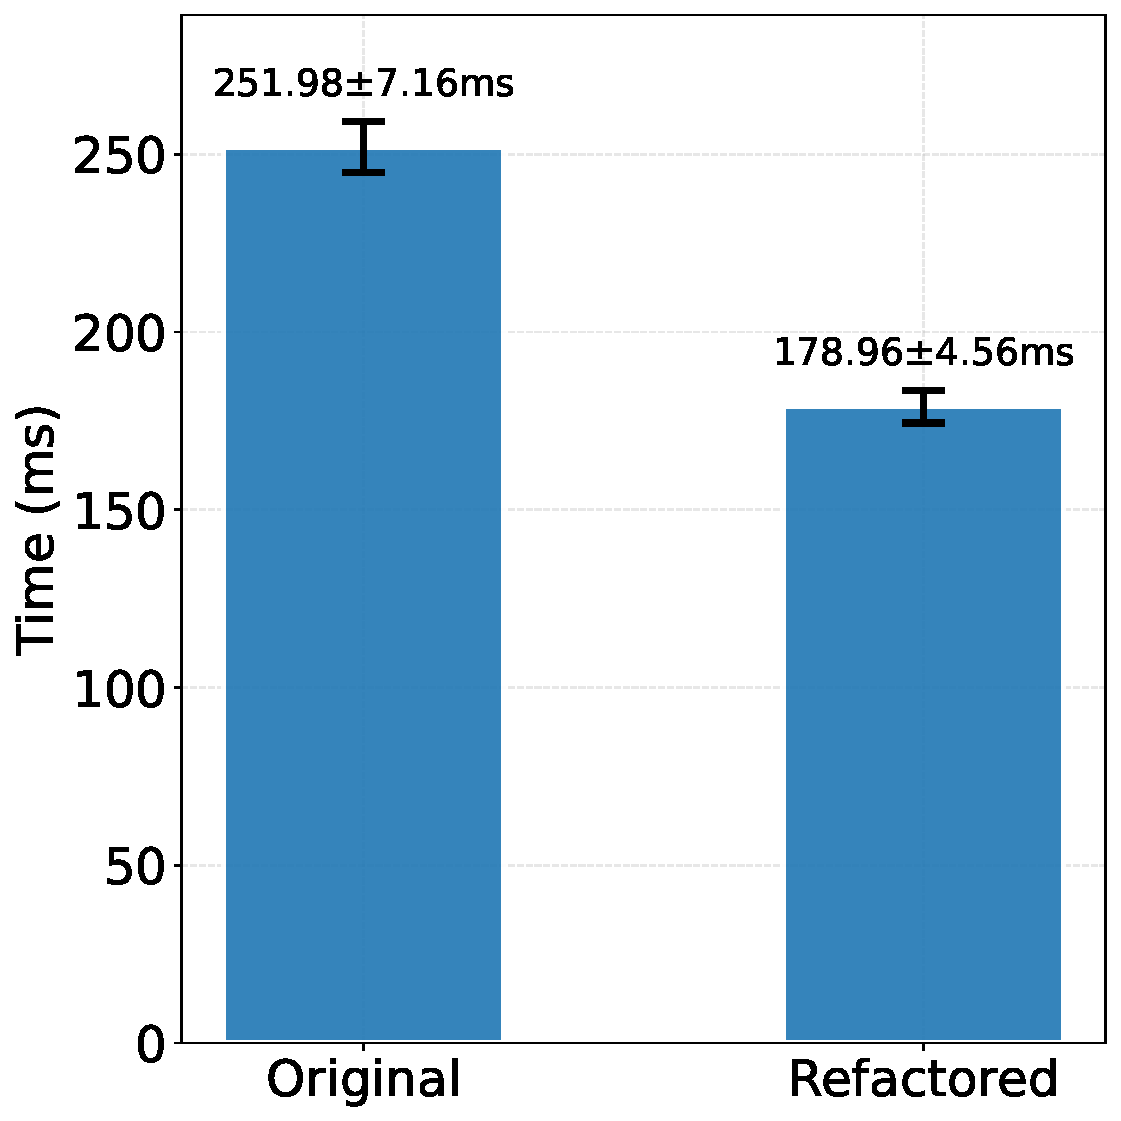
\includegraphics[width=0.35\textwidth]{timings_plot.pdf}
    \caption{Average prediction time of the original and refactored implementations. 
    Error bars represent the standard deviation across multiple runs. 
    The refactored implementation was observed to achieve a mean runtime of 
    178.96~$\pm$~4.56~ms compared to 251.98~$\pm$~7.16~ms for the original, 
    corresponding to a 1.41$\times$ speedup (approximately 29\% reduction in execution time).}
    \label{fig:timings}
\end{figure}

\section{Conclusion}
\label{sec:conclusion}

This project has contributed to the performance improvement and usability of the \texttt{MLPCpp} module in SU2. 
Through systematic profiling and targeted optimizations, key runtime bottlenecks were identified and 
addressed. The refactoring of the weight matrix storage, introduction of hash-based variable lookup, and 
improvements to the neural network compute functions resulted in a measurable reduction in execution 
time. Specifically, the optimized implementation achieved a mean prediction runtime of 
178.96~$\pm$~4.56~ms compared to 251.98~$\pm$~7.16~ms for the original version, corresponding to a 
1.41$\times$ speedup (approximately 29\% reduction in execution time). 

Beyond performance improvements, this work also contributed to the long-term maintainability of SU2. 
The integration of the Tracy profiler into the Meson build system, along with the accompanying 
documentation, ensures that future development within SU2 can benefit from low-overhead runtime 
analysis and continuous performance monitoring. 

\section{Future Work}
\label{sec:future}

Although several important optimizations were completed during this project, some work remains in progress 
and would benefit from further development. In particular, the migration of the weight matrix storage from 
a nested vector structure to a flattened vector representation is still under debugging. Completing this 
transition would allow the full benefits of contiguous memory storage to be realized in terms of performance 
and cache efficiency. 

Similarly, the proposed replacement of the \texttt{FindVariableIndices} function with a more direct and 
maintainable variable mapping approach requires additional testing and integration. Finalizing this change 
would improve both the clarity and the efficiency of variable lookups within \texttt{MLPCpp}. 

It is hoped that these ongoing efforts can be carried forward, building on the foundation established in this 
work and contributing to the long-term performance and maintainability of SU2.

\section{Acknowledgment}
\label{sec:ack}
I would like to sincerely thank Google and the SU2 community for providing me 
with the opportunity to contribute to this project through GSoC 2025. I am 
especially grateful to my mentors, Evert Bunschoten and Joshua A. Kelly, for their constant guidance, 
encouragement, and support throughout the project. Their approachable and 
friendly mentorship created an excellent learning environment, and their insights 
were invaluable in shaping the progress and outcomes of this work. I am also 
thankful to the wider SU2 developer community for their feedback, code reviews, 
and discussions, which greatly enriched the overall experience.


% \clearpage
\printbibliography

\end{document}

It is important to understand the arrangements of weights in the weight matrix of a Neural Network. Each row in the weight matrix represents all the incoming connections to one neuron in the output layer. It is made more clear by the illustration in Figure. 

It is important to discuss the elements in the weight matrix arrangement here because of the way it is used in the code. 

```Here the difference is th`at the indices in the weights mean it's from source to destination. While in the other one it meant it's from destination to source"

The \texttt{.mlp} files that contained the saved neural network by python tensorflow programs follow the arrangement of weights in the pattern as discussed above. And this is how they are loaded in the code. But for faster computations the indices are swapped and the weights are stored in a another container. Let's look below for why that is the case. 

There are indeed two independent \texttt{weights\_mat} variables, and they serve different purposes, following a clean separation of concerns:

\begin{enumerate}
    \item \texttt{CReadNeuralNetwork::weights\_mat}: This matrix exists within the \texttt{CReadNeuralNetwork} class, which acts as a temporary data reader and container. Its sole job is to parse the \texttt{.mlp} file and store the values, including the weights, exactly as they are structured in the file.

    \item \texttt{CNeuralNetwork::weights\_mat}: This matrix belongs to the \texttt{CNeuralNetwork} class, which represents the actual, functional neural network. This is the matrix that is used in the \texttt{Predict} method to perform the core mathematical operations (the dot products) of the network evaluation.
\end{enumerate}

You are also right about the data flow. The \texttt{CLookUp\_ANN::GenerateANN} method orchestrates this process perfectly:

\begin{enumerate}
    \item It creates a \texttt{CReadNeuralNetwork} object to read the file, which populates the first \texttt{weights\_mat}.
    \item It then loops through the layers and neurons, calling \texttt{Reader.GetWeight(...)} to retrieve the weights from the reader object and \texttt{ANN.SetWeight(...)} to populate the matrix in the functional \texttt{CNeuralNetwork} object.
\end{enumerate}

This is a good software design choice, as it cleanly separates the logic for parsing the file format from the logic of performing the neural network calculations.

\section*{Reason for Swapping Indices}

That's a brilliant insight, and you've hit on the exact reason. Yes, the swapping is almost certainly done for computational efficiency.

It all comes down to how CPUs access memory and a concept called data locality (or cache locality). In simple terms, CPUs are dramatically faster when they can read data from memory in a continuous, sequential block.

Let's look at the most critical calculation, the dot product inside the \texttt{ComputeX} function:

\begin{minted}{cpp}
// This loop is the computational core of the network
for (std::size_t jNeuron = 0; jNeuron < nNeurons_previous; jNeuron++) {
    x += weights_mat[iLayer - 1][iNeuron][jNeuron] *
         total_layers[iLayer - 1]->GetOutput(jNeuron);
}
\end{minted}

This loop calculates the input for a single destination neuron (\texttt{iNeuron}) by iterating through all the source neurons (\texttt{jNeuron}).

\subsection*{Why the [destination][source] Layout is Faster}

With the current \texttt{[layer][destination][source]} layout, all the incoming weights for a single destination neuron are stored next to each other in a contiguous block of memory.

When the loop runs, the CPU accesses the weights like this:
\begin{verbatim}
weights[dest_A][source_0]
weights[dest_A][source_1]
weights[dest_A][source_2]
...
\end{verbatim}

This is a sequential memory access pattern. When the CPU requests the first weight, it also loads the next several weights into its ultra-fast cache. For the next steps in the loop, the data is already in the cache, which is orders of magnitude faster than fetching from main memory. This results in a huge performance gain.